\chapter{Spezielle Methoden im Deep Learning}
Bereits zu Beginn (siehe Kapitel \ref{ch:DeepLearning}), wie auch im vergangenen Kapitel (siehe \ref{ch:cnn_model}) wurde darauf hingewiesen, dass Convolutional Neural Networks (CNNs) allgemeinen Multilayer Perceptrons (MLPs) in zwei zentralen Punkten überlegen sind. So reduzieren sie das Problem des \textit{Overfittings}, wobei es sich um die Überanpassung des Modells an die Trainingsdaten mit dem Resultat schlechter Generalisierung auf neue unbekannte Daten handelt. Dies geschieht durch Reduktion der freien Parameter und Verbindungen. Des Weiteren erlauben CNNs die lokale Extraktion von Merkmalen durch Einbezug räumlicher Korrelationen im Eingaberaum (vgl. \cite{LeCun1998}). 

Auch durch die Verwendung von CNNs bleiben dennoch zentrale Schwierigkeiten im Deep Learning bestehen:
\begin{itemize}
\item Verschwinden des Gradienten (\textit{Vanishing Gradient}) in tiefen Netzen (vgl. \cite{Hochreiter1991})
\item Gradientenabstieg bei nicht-konvexer Zielfunktion (vgl. \cite{Martens2010} und \cite{Dauphin14})
\item \textit{Overfitting} bei großen Netzen, insbesondere in nachgeschalteten MLPs (vgl. \cite{Hinton2012})
\item Schlechte Konditionierung der Fehlerlandschaft aufgrund von \textit{Parameter Sharing} (vgl. \cite{LeCun1998})
\end{itemize}

Die ersten beiden Problemen lassen sich unter der Problematik der sogenannten \textit{Pathological Curvature} zusammenfassen (vgl. \cite{Martens2010}). Historisch betrachtet liefert die Arbeit von \cite{Hochreiter1991} die Grundlage zu dem Problem, das heute als \textit{Vanishing Gradient}-Effekt bekannt ist. Dieser beschreibt den Zusammenhang zwischen der abnehmenden Größe des Fehlersignals und der Tiefe des Netzwerks. Das heißt, je mehr Hidden-Layer ein Netz besitzt, desto kleiner wird der Gradient in den vorderen Schichten und desto langsamer lernen diese Schichten in der Folge (siehe Abbildung \ref{fig:4_vanishing_gradient}).

\begin{figure}
\centering
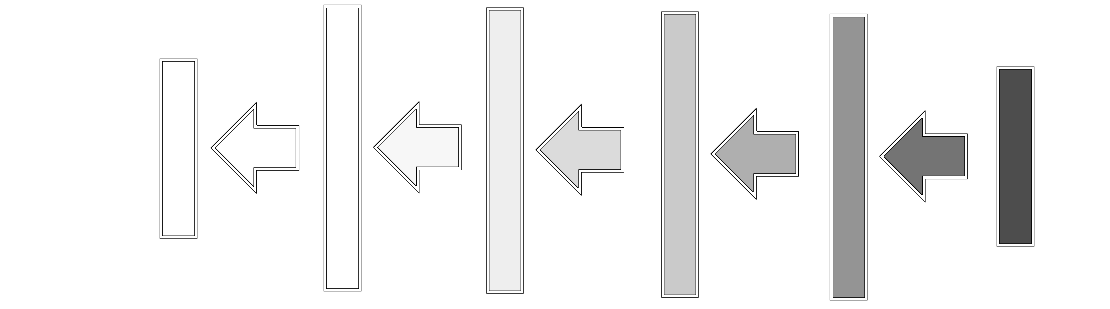
\includegraphics[width=0.7\linewidth]{images/4_vanishing_gradient}
\caption[]{Der Vanishing Gradient-Effekt beschreibt bei der Rückpropagierung das abklingende Fehlersignal von Output- hin zu Input-Layer}
\label{fig:4_vanishing_gradient}
\end{figure}

Deutlich wird der Effekt bei der Betrachtung der Formel \ref{eq:vanishgrad1} für das zurück\-propagierte Fehlersignal $\delta_{message}^l$ im Layer $l$, in der aus Kapitel  \ref{ch:cnn_back} bekannten $\delta_{message}$-Notation.
\begin{equation}
\label{eq:vanishgrad1} 
\delta_{message}^{l} = (W^{l})^T (\delta_{message}^{l+1} \circ \phi'(z^l))
\end{equation}
Setzt man klassische Aktivierungsfunktionen wie $sigmoid(\cdot)$ oder $tanh(\cdot)$ ein (siehe Kapitel \ref{ch:aktivierungsfunktonen}), gilt $\phi'(z^l) <= 1 $. Dies führt zwangsläufig zu einem abklingenden Fehlersignal (\textit{Vanishing Gradient}). Man könnte argumentieren, dass dies durch ein großes $W^l$, sodass $ (W^{l})^T (\delta_{message}^{l+1} \circ \phi'(z^l)) >= 1$, verhindert werden könnte. Dem ist nicht der Fall, da gleichzeitig $z^l = W^lx^l + b^l$ gilt und damit ein großes $W^l$ unweigerlich zu einem großen $z^l$ und damit zu einer kleineren Ableitung der Aktivierungsfunktion, welche ihr Maximum bei $0$ besitzt, führt. Ist zusätzlich zu einem großen $W^l$ der Schwellwert $b^l$ negativ, sodass $z^l \approx 0$, führt dies ebenso nicht zum Verschwinden des Effekts sondern zu einem, nicht weniger ungünstigen, \textit{Exploding Gradient}-Effekt. Selbst im linearen Fall ohne Aktivierungsfunktion tritt dieser Effekt auf, wenn die Gewichte jedes Neurons nicht die Norm $\|w\| \approx 1 $ besitzen.
 
Mit normalisierter Initialisierung der Gewichte lässt sich der Effekt kaschieren (vgl. \cite{Glorot2010}). Allerdings scheint erst die Verwendung der neuartigen ReLu-Aktivierungsfunktion (vgl. Kapitel \ref{ch:aktivierungsfunktonen}) den Effekt gänzlich zu unterdrücken und führt darüber hinaus zu oftmals erwünschten, dünnbesetzten (\textit{sparse}) Aktivierungen (vgl. \cite{Glorot2011}). Der Nachteil von ReLu-Neuronen ist allerdings, dass diese bei zu großen Lernraten und damit zu großen Änderungen der Gewichte unwiderruflich sterben (\textit{Dying ReLu}) und somit Teile des Netzes auslöschen können (vgl. \cite{Maas2013}).   

%http://people.idsia.ch/~juergen/fundamentaldeeplearningproblem.html original vanished gradients
\begin{equation} 
	f(x) =  max(0,x) 
\end{equation}


\begin{figure}
\centering
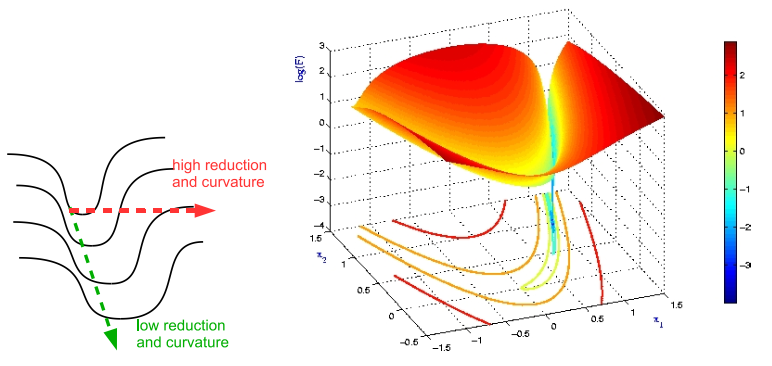
\includegraphics[width=0.7\linewidth]{images/4_pathological_curvature}
\caption[]{Pathological Curvature in der Rosenbrock-Funktion: $f(x,y = (1-x)^2 + 100(y -x^2)^2$ (vgl. \cite{Martens2010})}
\label{fig:4_pathological_curvature}
\end{figure}

Viele der in diesem Kapitel vorgestellten Methoden zielen auf den Vanishing-Gradient-Effekt ab, selbst wenn heute diskutiert wird, dass der Effekt nicht ausschließlich für die Schwierigkeiten im Deep-Learning verantwortlich ist. So zeigt \cite{Martens2010} empirisch, dass der Effekt ebenso auf eine ungünstige Fehlerlandschaft (\textit{Pathological Curvature}) zurückgeführt werden kann. Eine solche ist in Form der Rosenbrock-Funktion in Abbildung \ref{fig:4_pathological_curvature} dargestellt. 

Neben den benannten Problemen hinsichtlich der Fehlerfunktion, führt \textit{Overfitting} häufig ebenso zu schlechten Ergebnissen und entsprechende Regularisierungsmethoden werden benötigt.

\section{Vorverarbeitung}
%http://cs231n.github.io/neural-networks-2/
Der Bereich Vorverarbeitung steht nicht unmittelbar in Zusammenhang mit Deep Learning, wird jedoch zwecks der Vollständigkeit, besonders in Verbindung zu CNNs, vorgestellt.
\cite{Becker1991} stellte bereits Anfang der 90er Jahre fest, dass durch Dekorrelation der Trainingsdaten MLPs effizienter trainiert werden können. 
%Speeding up supervised learning. As Becker (1991) observes, if a representation with uncorrelated components is used as the input to a higher-level linear supervised learning network, then the Hessian of the supervised network's error function is diagonal, thus allowing efficient methods for speeding up learning (note that statistical independence is a stronger criterion than the mere absence of statistical correlation). Non-linear networks ought to profit as well.
\cite{LeCun1998b} fassen die klassische Vorverarbeitung in linearen MLPs wie folgt zusammen:
\begin{itemize}
\item Mittelwertfreie Trainingsdaten verhindern eine steile Fehlerlandschaft. 
\item Die Normalisierung der Varianz unterschiedlicher Merkmale verhindert deren unterschiedliche Gewichtung.
\item Die Dekorrelation der Trainingsdaten führt zwar zu einer diagonalen Hesse-Matrix, allerdings zeigt der Gradient nicht in Richtung Minimum. Dies muss durch dedizierte Lernraten, entsprechend den Kehrwerten der Eigenwerte pro Parameter, korrigiert werden.
\item Das Whitening der Daten führt zu einer kreisförmigen Fehlerlandschaft mit korrektem Gradienten.
\end{itemize}
Diese Hinweise gelten nur für lineare MLPs und somit quadratische Fehlerlandschaften. Die Fehlerlandschaft der hier verwendeten nicht-linearen MLPs kann jedoch lokal quadratisch approximiert werden (vgl. \cite{Hinton2015}).

Die genannten Techniken können allerdings nicht unmittelbar auf CNNs übertragen werden, da diese versuchen lokale Korrelationen an verschiedenen Orten im Eingaberaum zu extrahieren.
So zeigt sich bei der Verwendung von CNNs, dass die erfolgreichsten Architekturen lediglich den Mittelwert über die gesamten Trainingsdaten berechnen und diesen von jedem Pixel subtrahieren (vgl. \cite{Krizhevsky2012} und \cite{Simonyan2014}).
\cite{Kaparthy2014} kommen zu einem ähnlichen Schluss und beschreiben für CNNs lediglich die Zentrierung der Daten mittels globalen Mittelwert, alternativ pro Farbkanal oder Pixel, als nötige Vorverarbeitung. 
Teilweise werden für CNNs dennoch zwei weitere Techniken als Praxis beschrieben (vgl. \cite{Andrade2014} und \cite{Goodfellow_maxout_2013}) und deshalb im Folgenden kurz eingeführt.

\subsection{Kontrastnormalisierung}
Das Ziel der globalen Kontrastnormalisierung (GCN) ist es, unterschiedliche Trainingsbeispiele desselben Objekts in einen ähnlichen Kontrastbereich zu transformieren (vgl. \cite{Sermanet2012}). Die GCN bearbeitet jedes Trainingsbeispiel einzeln und berechnet den Mittelwert und die Varianz über alle Merkmale. Im Anschluss wird der Mittelwert subtrahiert und durch die Varianz geteilt. 

Neben der GCN wird häufig auch die lokale Kontrastnormalisierung (LCN) angewandt. Diese nimmt als Eingabe jeweils nur eine Umgebung $k_h \times k_w$ und berechnet die Kontrastnormalisierung in diesem Bereich \cite[vgl.][]{Sermanet2012}. 

Werden farbige Bilddaten im RGB-Raum verwendet muss bei diesem Verfahren beachtet werden, dass es zu einer Änderung des Farbtons kommen kann. Deshalb wird für Farbbilder entweder der HSV-Raum vorgeschlagen, in welchen nur die Intensität normalisiert wird \cite[vgl.][S. 56]{Pink2011}.
Oder es wird der YUV-Farbraum verwendet, und die Normalisierung lediglich auf den Y-Kanal angewandt \cite[vgl.][]{Sermanet2012}.

\subsection{ZCA-Whitening}
Der Begriff \textit{Zero Component Analysis} (ZCA) beschreibt ein der \textit{Principle Component Analysis} (PCA) sehr ähnliches Verfahren (vgl. im Folgenden \cite{Krizhevsky2009}). Es zielt darauf ab, die Eingangsdaten so zu dekorrelieren, sodass die Transformation so nahe wie möglich am Original ist. 

\begin{figure}[H]
\centering
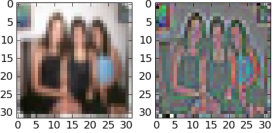
\includegraphics[width=0.5\linewidth]{images/4_ZCA}
\caption[]{Originales Bild (links) und ZCA-transformiertes Bild (rechts) (siehe. \cite{Krizhevsky2009})}
\label{fig:4_ZCA}
\end{figure}

Die Transformationsmatrix $W_{ZCA}$ ist in Gleichung \ref{eq:ZCA} angegeben, wobei die Kovarianzmatrix $C = X^TX$ ist. Der einzige Unterschied zum PCA-Whitening liegt darin, dass eine weitere Rotation zurück in den Bildraum durchgeführt wird. Dies ist möglich, da \textit{whitened-data} auch nach einer Rotation mit einer orthogonalen Matrix \textit{whitened} bleibt.

\begin{equation}
\label{eq:ZCA} 
W_{ZCA} = C^{-\frac{1}{2}} = P(D+\epsilon)^{-\frac{1}{2}}P^T = PW_{PCA}
\end{equation}

Abbildung \ref{fig:4_ZCA} zeigt die Transformation für ein Beispiel.


\section{Initialisierung}
Die Initialisierung eines neuronalen Netzes ist äußerst wichtig, da die Gewichte ungleich Null sein müssen. Ansonsten berechnen alle Neuronen die gleiche Ausgabe und somit die gleichen Gradienten. (\textit{Breaking the Symmetry}) \cite[vgl.][S. 201]{Rojas1996}.
\cite{LeCun1989} initialisieren die Gewichte beispielsweise zufällig zwischen $-\frac{2.4}{fan_{in}}$ und $\frac{2.4}{fan_{in}}$, wobei $fan_{in}$ der Anzahl Eingangsneuronen entspricht. Das hat zum Ziel die Nichtlinearität mit Werten um $0$ zu versorgen und damit nicht zu sättigen (\textit{Vanishing Gradient}).
Das erfolgreiche Netz von \cite{Krizhevsky2012} verwendet beispielsweise die Standard-Initialisierung, eine einfache Normalverteilung mit $W \sim \mathcal{N} (0,0.01)$. Dies ist möglich, da als Aktivierungsfunktionen ReLus verwendet werden, welche nicht sättigen können. 

Daneben existieren im Deep Learning heute zwei Arten zur Initialisierung, welche im Folgenden aufgeführt sind. 

\subsection{Normalisierte Fehlerpropagierung}
\begin{figure}
\centering
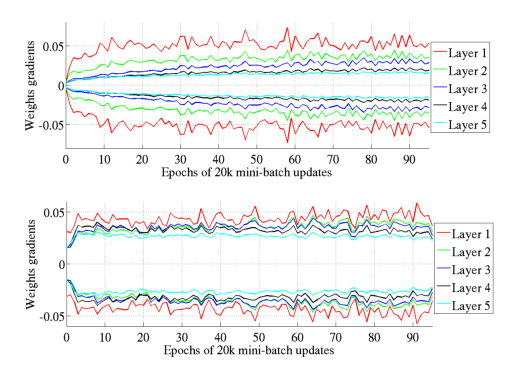
\includegraphics[width=0.7\linewidth]{images/4_xavier_init}
\caption[]{Vergleich der Varianz der Gradienten im Laufe des Trainings (Standard-Initialisierung (oben) und Xavier-Initialisierung (unten)): \textit{Layer 1} entspricht dem Output-Layer mit der größten Varianz im Gradient (siehe \cite{Glorot2010})}
\label{fig:4_xavier_init}
\end{figure}
Stellvertretend für eine derartige Initialisierung der Gewichte, sodass die Varianz des Signals sowohl bei der Berechnung der Ausgabe (\textit{forward pass}), als auch beim Zurückpropagieren des Fehlers (\textit{Backward Pass}) gleich groß bleibt  \cite[vgl. z.B.][S. 199 ff.]{Rojas1996}, steht heute die sogenannte \textit{Xavier-Initialization} (vgl. \cite{Glorot2010}). Dies führt dazu, dass die Varianz im Gradienten in jeder Schicht in etwa gleich groß ist, was aus Abbildung \ref{fig:4_xavier_init} zu entnehmen ist.
Die \textit{Xavier-Initialization} kombiniert beide Aspekte und initialisiert die Gewichte in der Art, dass die Varianz des Signals von Schicht zu Schicht sowohl im \textit{Forward Pass} als auch im \textit{Backward Pass} erhalten bleibt. Dies wird durch Formel \ref{eq:xavier} erreicht, was letztlich der Anwendung der Varianz-Formel für Gleichverteilung mit $Var(W) = \frac{2}{fan_{in}  + fan_{out}}$ entspricht.

\begin{equation}
\label{eq:xavier} 
W \sim \mathcal{U} [-\frac{\sqrt{6}}{\sqrt{fan_{in}  + fan_{out}}}, \frac{\sqrt{6}}{\sqrt{fan_{in}  + fan_{out}}}]
\end{equation}

Für den Fall, dass ReLu-Funktionen eingesetzt werden, verallgemeinert \cite{He2015} diese Formel insofern, dass eine lineare Approximation um $0$ für diese und davon abgeleitete Aktivierungsfunktionen nicht mehr gültig ist. Formel \ref{eq:xavier2} entspricht der Verallgemeinerung für Funktionen dieser Art. 

\begin{equation}
\label{eq:xavier2} 
W \sim \mathcal{N} (0,\sqrt{\frac{2}{fan_{out}}})
\end{equation}

Mit der Xavier-Initialisierung werden in Folge bessere Ergebnisse erreicht, als mit der Standard-Initialisierung (\textit{random initialization})in Verbindung mit Informationen 2. Ordnung (Appropximation der Hesse-Matrix - siehe. Kapitel \ref{ch:2norder}) (vgl. \cite{Chapelle11} und \cite{Glorot2010}).
Für Convolutional Neural Networks berechnet sich die \textit{$fan_{in}$} und \textit{$fan_{out}$} durch Multiplikation der Größe des rezeptiven Feldes mit der Anzahl \textit{Input-Maps}: $m \cdot k_w \cdot k_h$.


\subsection{Unüberwachtes Vortraining}
%- Pre-Training using Autoencoder/DNA					( 3 Seiten)	( 3 Seiten)
% two papers masci and ranzato 
Dieses Kapitel weicht die in Kapitel \ref{ch:Einleitung} gemachte Einschränkung auf das klassische überwachte, neuronale Lernmodell insofern auf, als dass ein unüberwachtes Lernverfahren vorgestellt wird. Dieses Vorgehen dient jedoch zum einen dem höheren Ziel, das überwachte Verfahren durch eine bessere Initialisierung der Parameter besser zu konditionieren und in der Performance zu verbessern. Zum anderen wird sich zeigen, dass es sich bei genauerer Betrachtung nicht um ein klassisches unüberwachtes Lernverfahren handelt: Es wird lediglich ein unüberwachtes Problem als überwachtes Problem angesehen. 
Dies lässt sich am einfachen Beispiel eines nichtlinearen Autoencoders verdeutlichen \cite[vgl. im Folgenden][]{Masci2011}. Der Encoder in Formel \ref{eq:autoenc1} nimmt als Eingabe einen Vektor $x \in \mathcal{R}^d$ und berechnet einen Code $h \in \mathcal{R}^{d'}$.
  
\begin{equation}
\label{eq:autoenc1} 
h = \phi(Wx + b)
\end{equation}

Dieser Code wird im zweiten Schritt durch den Decoder in Formel \ref{eq:autoenc2} dekodiert und so die Ausgabe berechnet. Das Ziel des Autoencoders ist es den Fehler zwischen Eingabe und Rekonstruktion, wie z.B. $MSE = \mathbb{E} [ (x - y)^2 ]$, durch Anpassen der Parameter $ \theta={W,b} $, wobei $W' = W^T$ (\textit{Tied Weights}), zu minimieren.
 
\begin{equation}
\label{eq:autoenc2} 
y = \phi(W'h + b')
\end{equation}

Der Autoencoder prädiziert folglich die Eingabe selbst und lernt die sogenannte Identität (\textit{Identity Mapping}).
Die Ideen von \cite{Hinton2006}, die gleichzeitig auch den Beginn der Renaissance von Deep Learning darstellen, beschreiben ein Verfahren große Netzwerke mit vielen Schichten \textit{greedy} schichtweise mit beschränkten Boltzmann Maschinen (RBMs) zu trainieren (vgl. \cite{Bengio2007}). Das heißt jede Schicht erhält als Eingabe die Ausgabe der vorherigen Schicht und versucht diese wiederum zu prädizieren (vgl. \cite{Ranzato2006}). Dies wirkt ähnlich einem Regularisierer und initialisiert die Parameter hinsichtlich Optimierung und Generalisierung in einer besseren Ausgangssituation \cite{Erhan2010}. Davon profitieren besonders große MLPs, welche bis dato aufgrund des \textit{Vanishing-Gradient}-Effekts für schwer zu trainieren galten. Eine wichtige Weiterentwicklung des Konzepts sind sogenannte \textit{Denoising Autoencoder} (DAs) bzw. \textit{Stacked Denoising Autoencoder} (SDAs). Diese versuchen die Eingabe $ x $ ausgehend von einer korrumpierten Version $ \hat{x} $ zu prädizieren. Dies erlaubt das Erlernen robuster Merkmale und kann als diskriminative Alternative zum generativen stochastischen RBM-Modell gesehen werden (vgl. \cite{Vincent2008}). 

Durch die besondere Struktur konnten Convolutional Neural Networks wie das \textit{LeNet 5} von \cite{LeCun1998} dennoch trainiert werden. Trotzdem ist es auch bei CNNs schwierig die ersten Schichten zu trainieren, da generell die hinteren Schichten schneller unscheinbares \textit{Overfitting} mit entsprechend kleinem Gradienten aufweisen (vgl. \cite{Erhan2010}). Der erste Versuch \textit{unsupervised pre-training} auf CNNs anzuwenden stammt von \cite{Ranzato2006}. Hier wird der erste Schicht eines veränderten \textit{LeNet 5} mittels Vortraining initialisiert, was den Fehler auf dem MNIST-Datensatz\footnote{Der MNIST-Datensatz handgeschriebener Ziffern besteht aus 60,000 Trainingsbeispielen und 10,000 Testbeispielen. Es stellt eine Untermenge des größeren NIST-Datensatzes dar. Die Bilder sind $28 \times 28$ und die Ziffern zentriert (\url{http://yann.lecun.com/exdb/mnist/} (26.08.2015)).} von $0.7 \%$ auf $0.6 \%$ verringert. Das Vortraining der $5 \times 5$-Filter geschieht mit zufällig gewählten $5 \times 5$-Bildausschnitten auf der Basis von RBMs.


\subsubsection{Convolutional Autoencoder}
\label{ch:autoenc}
Es existieren verschiedenste Architekturvorschläge für Autoencoder bzw. RBMs zum Vortraining von CNNs. Grundlage ist meist die Extraktion den Filter entsprechend großer Bildausschnitte und das Trainieren gewohnter Modelle (vgl. \cite{Desjardins2008}, \cite{Ranzato2007} oder \cite{Lee2009}).  
Im Folgenden wird der Convolutional Autoencoder von \cite{Masci2011} vorgestellt, da dieser auf Faltungen basiert und, wie Abbildung \ref{fig:4_mascii} zeigt, die gewünschten translations-invarianten Filter erzeugt. Die vorgestellte Variante verbessert den Fehler auf dem MNIST-Datensatz von $0.79 \%$ auf $0.71 \%$.

\begin{figure}
\centering
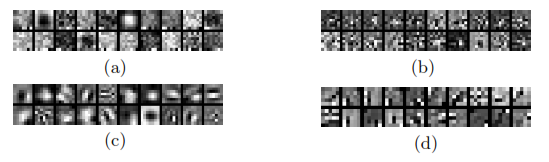
\includegraphics[width=0.7\linewidth]{images/4_mascii}
\caption[]{Filter der ersten Schicht eines Convolutional Autoencoders (a) Kein Max-Pooling, 0 \% Rauschen, (b) Kein Max-Pooling, 50 \% Rauschen, (c) Max-Pooling 2x2, (d) Max-Pooling 2x2, 30 \% Rauschen (siehe \cite{Masci2011})}
\label{fig:4_mascii}
\end{figure}

Die Architektur des vorgestellten Convolutional Autoencoders besteht aus einem Convolution-Layer sowie einem nachgeschalteten Pooling-Layer. Das bedeutet, der gesamte Autoencoder setzt sich letztendlich aus zwei hintereinander ausgeführte Layern dieser Art zusammen.

Gleichung \ref{eq:cautoenc1} zeigt die Berechnung des Codes $h_i$ der $i$-ten \textit{Feature-Map}. Dieser wird wie in gewöhnlichen CNNs durch Faltung mit Randbehandlung \textit{valid} berechnet. 

\begin{equation}
\label{eq:cautoenc1} 
h_i = \phi(\sum_{j=0}^{m}  x_{j} \ast W_{ij} + b_i)
\end{equation}

Der \textit{Decoder} berechnet die Funktion \ref{eq:cautoenc2}, wobei ähnlich dem \textit{backward pass} im Backpropagation die Filtermaske über beide Seiten geflippt bzw. um ($180^\circ)$ gedreht und die Randbehandlung (\textit{full}) verwendet wird. Die Dekodierung ist inspiriert von gewöhnlichen Autoencoder mit \textit{tied weights}, bei denen als Dekodierungsfunktion ebenso die transponierte Matrix des \textit{forward pass} verwendet wird.

\begin{equation}
\label{eq:cautoenc2} 
y_j = \phi(\sum_{i=0}^{n} h_{i} \ast rot180(W_{ij}) + c_j)
\end{equation}

Der Gradient für den Autoencoder berechnet sich mit Formel \ref{eq:cautoenc3}. Diese setzt sich, wie der Autoencoder, aus zwei Teilen zusammen. Der Erste für den \textit{Encoder}, der Zweite für den \textit{Decoder}. Im Unterschied zur Berechnung des Gradienten beim CNN wird statt $\delta y$ der Code $h$ der Flip-Operationen unterzogen. Dies tritt auf, da der \textit{Backward Pass} dem eigentlichen \textit{Forward Pass} entspricht.\footnote{Im Unterschied zur in \cite{Masci2011} beschriebenen Berechnung wird in Konsequenz auch auf die Flip-Operation von $\delta h$ nicht verzichtet und der Gradient am Ende gesamtheitlich geflippt. Der Gradient für den Encoder wird damit äquivalent zu dem in einem CNN berechnet. In Kapitel \ref{ch:debug} wird die Richtigkeit dieser Änderung überprüft.}
Eine zusätzliche Besonderheit existiert im Zusammenhang mit der Randbehandlung \textit{valid}. Um den Code $rot180(h)$ mit dem räumlich größeren $\delta y$ der Ausgabe zu falten, muss dieser doppelt \textit{Padding}  erhalten. Einmal um die gleiche Größe wie die Ausgabe zu erhalten und ein weiteres Mal um die Faltung zu ermöglichen.

\begin{equation}
\label{eq:cautoenc3} 
\frac{\partial J(W,b,c)}{\partial W_{ij}^l} = \frac{1}{M} \sum_{m=1}^{M} rot180(x_{mj}^l \ast  rot180(\delta h_{mi}^l) + rot180(h_{mi}^l) \ast \delta y_{mj}^l)   
\end{equation}

Analog zum bekannten Convolution-Layer berechnen sich die beiden Schwellwerte $b$ und $c$ aus der Summe der zugehörigen Deltas $\delta y$ und $\delta h$, wie in Gleichung \ref{eq:cautoenc4} und \ref{eq:cautoenc5} dargestellt.

\begin{equation}
\label{eq:cautoenc4} 
\frac{\partial J(W,b,c)}{\partial b_{i}^l} = \frac{1}{M} \sum_{m=1}^{M} \sum_{u=0}^{k_w} \sum_{v=0}^{k_w} \delta h_{miuv}^{l} 
\end{equation}


\begin{equation}
\label{eq:cautoenc5} 
\frac{\partial J(W,b,c)}{\partial c_{j}^l} = \frac{1}{M} \sum_{m=1}^{M} \sum_{u=0}^{k_w} \sum_{v=0}^{k_w} \delta y_{miuv}^{l} 
\end{equation}


Weiterentwicklungen wie die \textit{Tiled CNNs} versuchen weitere Filter-Invarianzen, beispielsweise Rotations-Invarianz, zu lernen (vgl. \cite{Quoc2010}).
Mit einer der größten Autoencoder, der \textit{Google Autoencoder} bedient sich ebenfalls der lokalen rezeptiven Feldern, verzichtet allerdings auf \textit{parameter sharing} um verschiedene Invarianzen zu lernen (vgl. \cite{LeRanzato2012}). Eine Schicht dieser Architektur ist in Abbildung \ref{fig:4_ranzato} abgebildet.

\begin{figure}
\centering
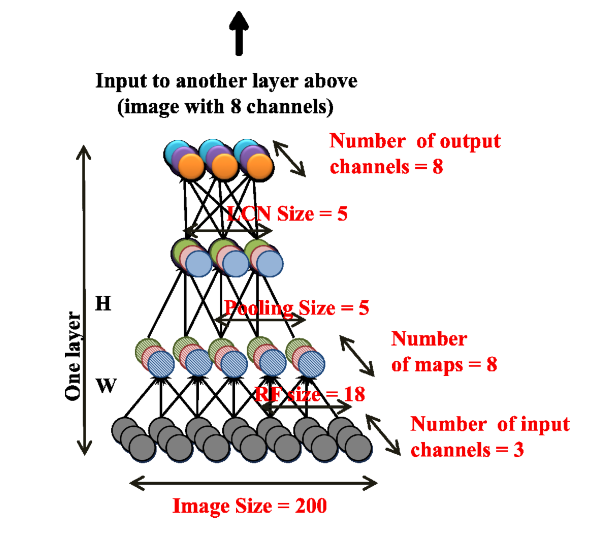
\includegraphics[width=0.5\linewidth]{images/4_ranzato}
\caption[]{Autoencoder mit lokalen rezeptiven Feldern und ohne \textit{parameter sharing} (\textit{non-convolutional}) (siehe \cite{LeRanzato2012})}
\label{fig:4_ranzato}
\end{figure}


Auch wenn das Verwenden von unüberwachtem Vortraining für die ersten Schichten eines CNNs attraktiv erscheinen, führt es nicht zu einer solchen Verbesserung der Ergebnisse als bei tiefen MLPs (DNNs) (vgl. \cite{Hamid2013}). 
Durch die Entwicklung neuer Aktivierungsfunktionen wie ReLu und raffinierter Initialisierung rückt das Thema somit weiter in solche Bereiche, in denen wenig gelabelte Trainingsdaten zur Verfügung stehen, das neuronale Netz vollständig überwacht zu trainieren (vgl. \cite{Masci2011} und \cite{LeRanzato2012}). Neben Aktivierungsfunktionen und Initialisierung tragen auch verbesserte Optimierungsverfahren zum Verschwinden von unüberwachtem Vortraining mit dem Ziel der besseren Initialisierung bei (vgl. \cite{Martens2010} und \cite{Sutskever2013}). 

Neuere Herangehensweisen zielen darauf ab, bereits trainierte CNNs für andere Probleme zu übernehmen, sogenanntes Transfer-Lernen (vgl. \cite{Wagner2013}). So liefert zum Beispiel die 7. Schicht des \textit{AlexNet} von \cite{Krizhevsky2012} gute Bildbeschreibungen (vgl. \cite{Bell2015}).


%http://stats.stackexchange.com/questions/163600/pre-training-in-deep-convolutional-neural-network
%There are some papers but not as much as autoencoders or RBMs. I think the reason is the time line of NN. Stacked RBM and autoencoder are introduced at 2006 and 2007, respectively. After employment of ReLU at 2009 unsupervised learning is partially abandoned (when there is enough data to learn in direct supervised learning). Even though Convolution net (or LeNet) is invented at 1989, it couldn't trained as deep structure till 2012 which is after popularization of direct supervised learning with ReLU. So researchers, I guess, have trained it mostly by using direct supervised learning.

%Whereas theoretical work suggests that deep architectures
%might be more efficient at representing
%highly-varying functions, training deep architectures
%was unsuccessful until the recent advent
%of algorithms based on unsupervised pretraining.
%Even though these new algorithms have
%enabled training deep models, many questions
%remain as to the nature of this difficult learning
%problem. Answering these questions is important
%if learning in deep architectures is to be further
%improved. We attempt to shed some light
%on these questions through extensive simulations.
%The experiments confirm and clarify the advantage
%of unsupervised pre-training. They demonstrate
%the robustness of the training procedure
%with respect to the random initialization, the positive
%effect of pre-training in terms of optimization
%and its role as a regularizer. We empirically
%show the influence of pre-training with respect to
%architecture depth, model capacity, and number
%of training examples
%\cite{Erhan2010}

% direct learning and outlook to learning with constraints
%\cite{Zeiler2011} % Not stacked

%Local contrast Normalisierung ebenso good presentation nips 
\section{Gradientenabstieg}
\label{ch:gradient}
%Picture
%http://blog.datumbox.com/tuning-the-learning-rate-in-gradient-descent/
%Alternative Stochastic Gradient Descent tricks picture
%Unlike LMS / SVM / etc. which are linear in parameter
%neuronale netze nicht linear in parameter
\begin{figure}
\centering
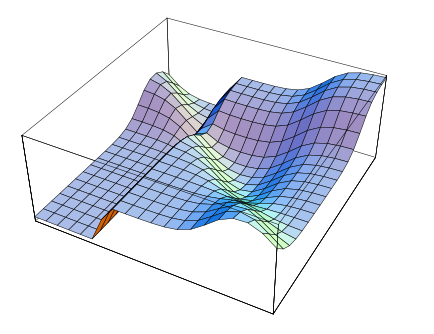
\includegraphics[width=0.5\linewidth]{images/4_Gradient2}
\caption[]{Fehlerfunktion bzw. Zielfunktion im Parameterraum mit lokalem Minimum \cite[siehe][S. 155]{Rojas1996} }%\cite[siehe][Kap. 5, S. 17]{Duda2001}}
\label{fig:4_Gradient}
\end{figure}
Dieses Kapitel behandelt verschiedene Methoden zur Verbesserung des Gradientenabstiegs. Diese können das Training erheblich beschleunigen, da es sich im Allgemeinen im Deep Learning um nicht-konvexe Fehlerlandschaften wie in Abbildung \ref{fig:4_Gradient} handelt.

%			- Learning rate via SVD
%			- Con
Grundlage für das effiziente Lernen mit vielen Trainingsdaten ist der sogenannte stochastische Gradientenabstieg (SGD)(vgl. im Folgenden \cite{Bottou1998}). Dabei geht es um die Frage, wie die erwartete durchschnittliche Richtung des Gradienten ist. Durch die Einführung des MSE-Fehlermaß ist der Ansatz des SGD bereits gegeben. So entspricht die MSE-Fehlerfunktion dem Erwartungswert einzelnen Fehlerquadrate. Wie in Gleichung \ref{eq:sgd_mse} zu sehen ist, entspricht dazu analog der Erwartungswert der einzelnen Gradienten dem Gradient der Fehlerfunktion.

\begin{equation}
\label{eq:sgd_mse} 
\nabla J(W,b) =  \mathbb{E}[\nabla (f(x_i) - y_i)^2] = \frac{1}{N}\sum_{i}^{N} \nabla (f(x_i) - y_i)^2
\end{equation}

Für eine allgemeine Fehlerfunktion $e(x)$ gilt: Nimmt man an Stelle der gesamten Trainingsmenge $N$ (\textit{Batch}) eine repräsentative Teilmenge $M$ oder auch einzelne Trainingsbeispiele $i$ (\textit{Online}), so ergibt sich Formel \ref{eq:sgd} für den Gradientenabstieg mit Lernrate bzw. Schrittweite $\eta$. Der Gradient zeigt so in Richtung des Durchschnitts und damit immer in der Erwartung in die richtige Richtung. Üblicherweise werden die so für die Berechnung entnommenen Teilmengen als \textit{Mini-Batch} bezeichnet. Neben einem günstigeren Rechenaufwand liefert SGD eine Zufallskomponente (\textit{Randomization}), welche zu beschleunigter Konvergenz führen kann und die Möglichkeit des Trainings ohne unmittelbarem Zugriff auf die gesamte Trainingsmenge. 

\begin{equation}
\label{eq:sgd} 
W_{t+1} = W_t - \eta \frac{1}{M} \sum_{i=1}^{M} \nabla e(x_i)
\end{equation}

SGD bildet die Grundlage für viele Erweiterungen und stellt so die erste Optimierung des Gradientenabstiegs dar. 
Um die Formeln zu vereinfachen wird im Folgenden auf die Mittelung des Gradienten verzichtet und an den entsprechenden Stellen darauf hingewiesen, ob es sich die Erweiterung für den Mini-Batch-Modus oder den klassischen Batch-Modus, welcher für Deep Learning in Verbindung mit vielen Trainingsdaten unpraktikabel ist, handelt. 

\subsubsection{Lernrate}

Wird der klassische Gradientenabstieg ohne Optimierungen verwendet ist es besonders wichtig $\eta$ richtig zu wählen. Aufgrund des \textit{Vanishing Gradients} sollte die Lernrate in den letzten Schichten kleiner gewählt werden. Außerdem ist darauf zu achten, dass durch \textit{Parameter Sharing} die Lernrate proportional zur Wurzel der Verbindungen ist, die sich einen Parameter teilen (vgl. \cite{LeCun1998b}). Letzteres ist gerade hinsichtlich CNNs zu beachten, um eine unnötig schlechte Konditionierung der Fehlerlandschaft zu vermeiden.


\subsection{Momentum}
Eine der ersten erfolgreichen Erweiterung zum Backpropagation ist die sogenannte Momentum Methode von \cite{Polyak1964}.
Die Momentum-Methode ist durch die Physik motiviert, indem dem Gradienten eine potentielle Energie zugewiesen wird. Dies erlaubt es in gleichbleibender Richtung des Gradienten Geschwindigkeit aufzunehmen, was letzten dazu führt, dass in flachen Regionen der Fehlerlandschaft größere und in unwegsamen Bereichen kleinere Schrittweiten effektiv ausgeführt werden (vgl. \cite{LeCun1998b}).
Dies wird durch Hinzufügen eines weiteren durch Terms in das Gewichtsupdate erzielt. Wie Formeln \ref{eq:momentum} und \ref{eq:momentum1} zeigen bildet die Momentum-Methode einen gewichteten Durchschnitt der vergangenen Gradienten der Gewichte. 
 
\begin{equation}
\label{eq:momentum} 
\Delta W_t = \mu \Delta W_{t-1} - \eta \nabla J(W_t,b_t)
\end{equation} 
 
\begin{equation}
\label{eq:momentum1} 
W_{t+1} = W_t + \Delta W_t
\end{equation}

Typische Parametrisierung für die Momentum-Rate $\mu$ sind Werte größer $0.9$. Diese sind allerdings abhängig von Lernproblem und können nicht allgemein formuliert werden (vgl. \cite{Kaparthy2014}). Momentum ist die einfachste Optimierung für SGD und findet selbst in großen Netzen häufig Anwendung (vgl. \cite{Krizhevsky2012}).

\subsubsection{Nesterov-Methode}
Die Nesterov-Methode (NAG) ist eine verbesserte Momentum-Methode, die von \cite{Nesterov1983} inspiriert ist \cite[vgl. im Folgenden][]{Sutskever2013b}. Diese Methode führt zuerst den über die vergangenen Perioden gewichteten Momentum-Term aus und berechnet den Gradient an dieser Stelle. Die Methode fungiert so als eine Art Ausblick auf die zukünftige Fehlerlandschaft. Der eigentliche Gradient ergibt sich schließlich aus Ausblick und Korrektur, wie Abbildung \ref{fig:4_nesterov} zeigt.
\begin{figure}
\centering
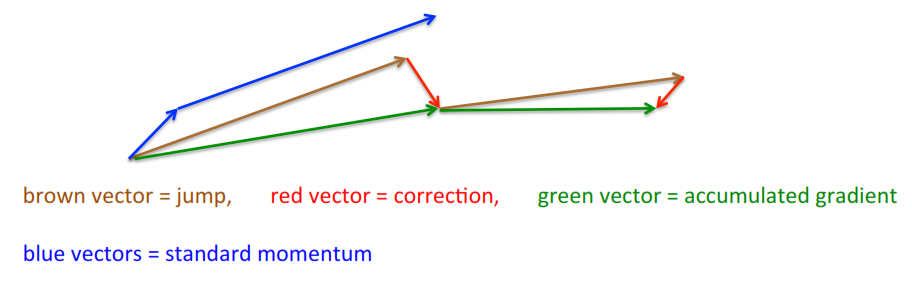
\includegraphics[width=0.7\linewidth]{images/4_nesterov}
\caption[]{Das effektivere Nesterov-Momentum korrigiert Fehler im Nachhinein\cite[siehe][]{Hinton2015} }%\cite[siehe][Kap. 5, S. 17]{Duda2001}}
\label{fig:4_nesterov}
\end{figure}

Da diese Ausführung die Reihenfolge des üblichen Trainings beeinflussen würde, wird die Methode derart umgeschrieben, dass die aktuellen Parameter immer dem Ausblick entsprechen. Daraus ergeben sich folgende Regeln \ref{eq:nesterov1} und \ref{eq:nesterov2} für die Aktualisierung der Gewichte (vgl. \cite{Kaparthy2014}).


\begin{equation}
\label{eq:nesterov1} 
\Delta W_t = \mu \Delta W_{t-1} - \eta  \nabla J(W_t,b_t)
\end{equation}
\begin{equation}
\label{eq:nesterov2} 
W_{t+1} = W_t + (-\mu \Delta W_{t-1} ) + (1 + \mu) \Delta W_t
\end{equation}

Die beschriebene Methode ist robuster gegenüber der Momentum-Rate und lässt höhere Raten zwischen $0.95$ und $0.99$ zu. NAG wird viel Potential zugesprochen das klassische Momentum dauerhaft zu ersetzen (vgl. \cite{Sutskever2013}).


\subsection{Adaptive Lernrate}
\label{ch:2norder}
Ein allgemeines Problem in Verbindung von Gradientenabstieg und dem Training im Deep Learning ist der $Vanishing Gradient $-Effekt \cite{Hochreiter1991}. Ein Algorithmus der direkt auf diesen Effekt abzielt, ist der sogenannte Resilient Propagation, oder auch Rprop genannt (vgl. \cite{Riedmiller1992} und \cite{Igel2000}). Rprop weist jedem Parameter eine eigene Lernrate zu und verzichtet gänzlich auf die Werte des Gradienten. Die grundlegende Arbeitsweise sieht vor bei gleichbleibendem Vorzeichen einer partiellen Ableitung wird die zugehörige Lernrate mit erhöht. Tritt ein Vorzeichenwechsel liegt es nahe, dass in der Richtung dieser Ableitung eine Senke übersprungen wurde und die Lernrate reduziert. Rprop ist äquivalent zum Gradientenabstieg, wenn bei letzterem durch die Länge des Gradient geteilt wird.
Hier liegt ein fundamentales Problem hinsichtlich Deep Learning: Um die Länge des Gradients zu schätzen, bedarf es der gesamten Trainingsmenge, was die Verwendung von SGD ausschließt. Somit ist Rprop nur für Offline-Training geeignet (vgl. \cite{Hinton2015}).



Der bekannte allgemeine Newton-Algorithmus für Optimierung in Gleichung \ref{eq:hessianstep} multipliziert an Stelle einer globalen Lernrate mit der Inversen der Hesse-Matrix. Unter bestimmten Annahmen wie z. B. einer quadratischen Zielfunktion erreicht dieser Algorithmus innerhalb eines Schrittes das Minimum, was als Newton-Schritt bezeichnet wird (vgl. \cite{Bottou1998}).

\begin{equation}
\label{eq:hessianstep} 
W_{t+1} = W_t - H_t^{-1} \frac{1}{M} \sum_{i=1}^{M} \nabla J(W_t,b_t)
\end{equation}

Die Hesse-Matrix ist im Allgemeinen sehr teuer zu berechnen, da jede partielle Ableitung der Parameter $N$ nochmals abgeleitet werden müsste. Dies führt auf eine $N \times N $-Matrix, welche in neuronalen Netzen nicht effizient zu berechnen ist und deshalb approximiert werden muss \cite[vgl.][]{LeCun1998b}. 
Algorithmen mit sogenannter adaptiver Lernrate gehen so vor, dass sie lediglich die Diagonale der Hesse-Matrix $diag(H)^{-1}$ approximieren. Dies führt zu eigenen Lernraten pro Parameter, welche idealerweise den echten Eigenwerten der Hesse-Matrix entsprechen \cite[vgl.][]{LeCun1998b}. Adaptive Lernraten erlauben Schrittweiten in Gegenden schwacher Krümmung zu erhöhen und entsprechend in anderen zu verkürzen. Dieser Mechanismus wirkt damit ebenso unmittelbar dem \textit{Vanishing Gradient}-Effekt entgegen, da kleiner werdende Gradienten zu den ersten Schichten hin skaliert werden \cite[vgl.][]{Martens2010}. 
Problem bei der Verwendung der Hesse-Matrix für nicht-konvexe Probleme sind negative Eigenwerte an lokalen Maxima oder gemischt positive und negative Eigenwerte an Sattelpunkten, die zu einer falschen Richtung des Gradienten führen \cite[vgl.][]{Dauphin14}. Aus diesem Grund ist es notwendig eine Methode mit entsprechender Vorkonditionierung zu verwenden \cite[vgl.][]{Dauphin2015}.


\subsubsection{Stochastic Levenberg-Marquardt}
Der bekannte stochastische Levenberg-Marquardt-Algorithmus (LMA) von \cite{LeCun1998b} ist ein Algorithmus im Bereich Neuronale Netze und SGD, der direkt versucht die $diag(H)$ zu approximieren. Zwei weitere Approximationen sind dazu allerdings notwendig. So wird die  Gauß-Newton-Approximation zur Vermeidung negativer Eigenwerte, wie im klassischen Levenberg-Marquardt-Algorithmus, angewandt und die $diag(H)$ nur auf einer kleinen Teilmenge der Trainingsdaten berechnet. Darüber hinaus wird die Berechnung nur einmal pro Epoche durchgeführt. Da die Kosten einem normalen \textit{forward pass} sowie einem angepassten \textit{backward pass} der zur Rückpropagierung der zweiten Ableitungen dient, sind diese zu vernachlässigen. 
Neben der Kompensation des \textit{Vanishing-Gradients}, kompensiert der stochastische (LMA) den Effekt der schlechten Konditionierung der Fehlerlandschaft durch \textit{Parameter Sharing} \cite[vgl.][]{LeCun1998b}.
Die neue Lernrate pro Parameter $i$ ergibt sich mit Formel \ref{eq:lma}.

\begin{equation}
\label{eq:lma} 
\eta_{i} = \frac{\eta}{\mu + H_{ii}}
\end{equation}

Wie im klassischen LMA wird ein Dämpfungsfaktor $\mu$ verwendet, um zu verhindern, dass die Schrittweite zu groß wird. Dieser Faktor kann auch als $l_2$ a-priori Annahme gesehen werden, die angibt, dass sich das Gewicht nicht ändern soll, wenn die Krümmung entsprechend klein wird (vgl. \cite{Martens2010}). Im \textit{LeNet 5} wird $\mu = 0.02$ verwendet.


\subsubsection{Equilibrium SGD}
Eine Verbesserung zum stochastischen LMA ist die von \cite{Dauphin2015} beschriebene Equilibrium-Methode, welche die Matrix $D^{Eq} = \sqrt{diag(H^2)})$ berechnet. Diese Vorkonditionierung bietet einige Vorteile hinsichtlich der Behandlung der genannten indefiniten Hesse-Matrizen, aufgrund von Sattelpunkten innerhalb der Fehlerlandschaft von MLPs. Darüber hinaus kann diese Methode effizient durch den Zusammenhang in Formel \ref{eq:equi} mit $v \sim \mathcal{N} (0,1)$, beispielsweise mit $R\{\cdot\}$-Operator (vgl. \cite{Pearlmutter1994}), berechnet werden. 

\begin{equation}
\label{eq:equi} 
D^{Eq} = diag(H^2) = E[(Hv)^2]
\end{equation}

Im Unterschied zum stochastischen LMA bildet die Equilibrium-Methode einen mit $\rho$ gewichteten \textit{root mean square}-Durchschnitt (RMS) über die vergangenen Perioden wie Formel \ref{eq:equi1} zeigt. \cite{Dauphin2015} schlagen eine Neu-Berechnung von $D^{eq}$ nach jeweils 20 Iterationen vor und $\mu = \{10^{-4},10^{-5},10^{-6}\}$.

\begin{equation}
\label{eq:equi1} 
D^{eq}_{t+1} = \rho D^{eq}_{t} + (1 - \rho) (Hv)^2
\end{equation}

Damit ergibt sich eine die in Formel \ref{eq:equi2} gezeigte effektive Lernrate, welche ebenfalls einen Dämpfungsfaktor $\mu$ zur Vermeidung großer Schrittweiten beinhaltet.

\begin{equation}
\label{eq:equi2} 
\eta_{i} = \frac{\eta}{\mu + \sqrt{D^{eq}_{ii}}}
\end{equation}

\subsubsection{RMSprop}
RMSprop stammt von \cite{Hinton2015} und kombiniert zwei Ideen. Einerseits verarbeitet er die Idee des Rprop nur auf das Vorzeichen des Gradienten zu achten, in dem er den \textit{root mean square}(RMS) Durchschnitt der partiellen Ableitungen berechnet. Andererseits behebt er dadurch das Hauptproblem von AdaGrad stetig die effektive Lernrate zu verkleinern \cite[vgl.][Kap. 8.4.1, S. 257]{Bengio2015}. Die Berechnung von RMS geschieht gemäß Formen \ref{eq:rmsprop1}. Die effektive Lernrate berechnet sich so wie in Formel \ref{eq:rmsprop2} dargestellt, wobei ebenfalls ein Dämpfungsfaktor $\mu$ verwendet wird.

\begin{equation}
\label{eq:rmsprop1} 
\hat{H}_{t+1} = \rho \hat{H}_{t} + (1 - \rho) \nabla J(W_t,b_t)^2
\end{equation}


\begin{equation}
\label{eq:rmsprop2} 
\eta_{i} = \frac{\eta}{\mu + \sqrt{\hat{H}_{ii}}}
\end{equation}

RMSprop stellt eine sehr effektive und praktische Optimierung dar, welche dazu einfach zu implementieren ist. Dies macht diese derzeit sehr beliebt (vgl. \cite{Bengio2015}). Eine weitere sehr interessante Eigenschaft von RMSprop ist die Fähigkeit zur Approximation der Equilibrium-Matrix $D^{Eq} = \sqrt{diag(H^2)})$ (vgl. \cite{Dauphin2015}).

\subsubsection{AdaDelta}
AdaDelta ist eine von \cite{Zeiler2012} entwickeltes Verfahren, das ebenfalls das Problem der immer kleiner werdenden Lernrate von AdaGrad adressiert (vgl. \cite{Bengio2015}). Dazu versucht AdaDelta Informationen über die Krümmung (\textit{second-order gradient information}) aus der ersten Ableitung zu berechnen. Der Divisior in Formel \ref{eq:adadelta1} entspricht, bis auf das unter der Wurzel stehende $\mu$, dem des RMSprop. Neu ist der quadratische Mittelwert über $MS[\Delta x]$, der einen Zeitschritt versetzt berechnet wird und als eine Art Momentum wirkt.


\begin{equation}
\label{eq:adadelta1} 
\Delta x_{t} = \frac{\sqrt{\mu + MS[\Delta x]_{t-1} }}{\sqrt{\mu + H_{t}}} 
\end{equation}

Die effektive Lernrate ergibt sich mit Formel \ref{eq:adadelta3}.

\begin{equation}
\label{eq:adadelta3} 
 \eta_{i} = \Delta x_i
\end{equation}

Das Interessante an AdaDelta ist, dass es gänzlich auf eine globale Lernrate verzichtet und lediglich $\mu$ als Hyperparameter benötigt. Da sich $\mu$ unter der Wurzel findet ist dieses entsprechend etwas kleiner als bei den vorherigen Methoden. \cite{Zeiler2012} schlägt Werte bis $\mu = 10^{-8}$ vor.


\subsection{Hessian free optimazation (HF)}
\label{ch:hf}

Algorithmen mit adaptiver Lernrate lassen im Sinne der Approximation alle nicht-diagonalen Werte der Hesse-Matrix weg. Damit wird ein gewisser Fehler in Kauf genommen, da diese Werte gerade die Interaktion der Parameter hinsichtlich der Zielfunktion beschreiben (vgl. \cite{Martens2010}). 

Die \textit{Hessian free optimazation} (HF) von \cite{Martens2010} versucht im Gegensatz zu den vorherigen Methoden nicht den \textit{Vanishing Gradient}-Effekt zu eliminieren, sondern zielt direkt auf die Optimierung von Fehlerlandschaften mit \textit{Pathological Curvature} ab.
Für eine gegebene Stelle $w_t$ im Parameterraum wir ein lokales quadratisches Modell angenommen und dieses mittels Conjungate Gradient (CG) optimiert. Damit kann HF nur im \textit{Batch}-Modus betrieben oder analog zum stochastischen LMA mit hinreichend großer Teilmenge der Trainingsdaten. Eine Besonderheit ist, dass die Methode den gefundenen Vektor von CG im letzten Zeitschritt als Initialisierung für den aktuellen Zeitschritt wählt und dadurch Informationen über mehrere Iterationen weitergeben kann.
Kritisch betrachtet ist diese Methode durch die Verwendung des linearen CG keine Methode zweiter Ordnung und dadurch den anderen Methoden nicht allgemein überlegen. So zeigt \cite{Sutskever2013}, dass die vorgestellte HF-Methode sehr viele Ähnlichkeiten zum Nesterov-Momentum aufweist und zu diesem unter der Annahme, dass nur ein Schritt im CG-Algorithmus ausgeführt wird, sogar äquivalent ist. 

Die wichtige Eigenschaft der beiden Methoden, HF und NAG, ist die Fähigkeit die Schrittweiten in Bereichen mit wenig Krümmung zu erhöhen und entsprechend zu verringern in Bereichen hoher Krümmung. Damit wird der NAG-Methode gerade im Bereich tiefer Netze hohes Potenzial zugesprochen (vgl. \cite{Sutskever2013}).

					

\section{Regularisierung und Generalisierung}
% 
%	- Regularization									( 4 Seiten)			
%		- Baysian viewpoint on regularization
%	- Maschinelles Lernen
%		- Lernen einer Funktion R^n -> R^m
%		- Function Viewpoint
%		- Data Viewpoint
%		- Basian view = ridge regression 
%		- Least Squares Viewpoint + regularization
%		- Dual form ridge regression + gaussian process


Das Lernproblem selbst lässt sich beispielsweise mit bayesianischer Inferenz (siehe \ref{eq:bayesParam}) anschaulich beschreiben \cite[vgl. im Folgenden][S. 159f]{Mitchell1997}.
\begin{equation}
\label{eq:bayesParam}
P(h|\mathcal{D}) = \frac{P(\mathcal{D}|h)P(h)}{P(\mathcal{D})}
\end{equation}
Die Formel beschreibt den Zusammenhang zwischen gegebenen Trainingsdaten $\mathcal{D}$ und der Hypothese $h$, welche den zu erlernenden Parametern  $\Theta = \{W,b\} $ entspricht. Diese soll die gegebenen Daten $\mathcal{D}$ möglichst gut abbilden können sowie eine gute Generalisierung für unbekannte Daten leisten. In der bayesianischen Interpretation korrespondieren Regularisierer mit der A-priori Verteilung der Hypothese $h$ \cite[vgl. im Folgenden][Kap. 7, S. 196]{Bengio2015}.
Im Deep Learning existieren verschiedenste Methode der Regularisierung mit dem Ziel der besseren Generalisierung. Manche betreffen die Parameter selbst, andere codieren Expertenwissen oder regulieren die Kapazität von Modellen mit sehr vielen freien Parametern. 
Im Umfeld neuronaler Netze betrifft die Regularisierung von Parametern meist lediglich $W$ und der Schwellwert $b$ bleibt unbeachtet.
					

\subsection{A-priori Annahmen}

Die A-priori Verteilung der Parameter $\Theta$ gibt an wie Wahrscheinlich verschiedene Werte dieser sind. Die klassischen Methoden des maschinellen Lernens sowie der Statistik bestrafen die Norm der Parameter (\textit{Parameter Norm Penalty}). Die Norm wird als $\Omega(\Theta)$ definiert und zur Zielfunktion, wie in Gleichung \ref{[eq:reg1]}, gewichtet mit dem Hyperparameter $\alpha$ addiert \cite[vgl.][Kap. 7.2, S. 200]{Bengio2015}. 

\begin{equation}
\label{[eq:reg1]}
\hat{J}(W,b) =  J(W,b) + \alpha \Omega(\Theta)
\end{equation}

Typische Normen sind die $L^1$- und $L^2$-Norm. Abbildung \ref{fig:4_regularizer} stellt die beiden Varianten gegenüber.

\begin{figure}
\centering
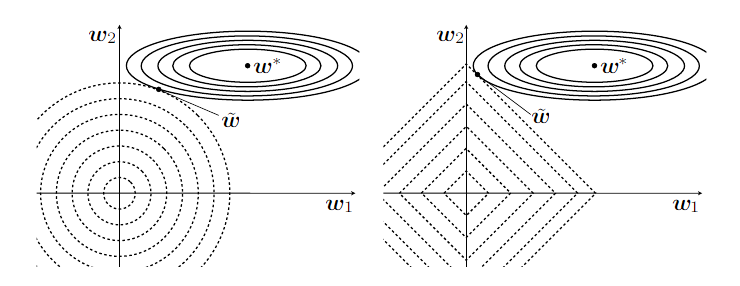
\includegraphics[width=0.8\linewidth]{images/4_regularizer}
\caption[]{Effekt von $L^2$- (links) und $L^1$-Norm (rechts) auf den Wert der optimalen Parameter $W$ mit empirischem Optimum $W^*$ \cite[vgl.][Kap. 7.2, S. 199]{Bengio2015} }.
\label{fig:4_regularizer}
\end{figure}


\subsubsection{$L^1$-Norm}

Bei der Verwendung der $L^1$-Norm zur Berechnung von $\Omega{\Theta}$ bleibt nach Ableiten lediglich noch das Vorzeichen $sign(w_i)$ der einzelnen Parameter übrig. Damit ergibt sich die in Gleichung \ref{eq:reg1} dargestellte Regel für die Berechnung des neuen Gradienten $\nabla_w \hat{J}(W,b)$ pro Parameter $w$. 

\begin{equation}
\label{eq:reg1}
\nabla_w \hat{J}(W,b) = \nabla_w J(W,b) + \alpha sign(w)
\end{equation}

Die $L^1$-Regu\-lari\-sierung bestraft die Summe aller Absolutwerte der Parameter und verkleinert diese während des Gradientenabstiegs somit stetig mit gleicher Rate. Die rechte Grafik in Abbildung \ref{fig:4_regularizer} zeigt, dass $L^1$-Regu\-lari\-sierung zu sowohl größeren als auch kleineren Werten führt. Diese Eigenschaft führt zu \textit{Sparsitiy}, da kleine Parameter $w$ zwangsläufig zu null gemacht werden \cite[vgl.][Kap. 7.2, S. 203]{Bengio2015}.
Die bayesianische Interpretation der Methode ist die A-priori Annahme einer isotropischen Laplace-Verteilung der Parameter \cite[vgl.][Kap. 7.2, S. 206]{Bengio2015}.


%http://www.iro.umontreal.ca/~bengioy/DLbook/regularization.html


%http://www.chioka.in/differences-between-l1-and-l2-as-loss-function-and-regularization/
%		- L1 / L2 ( Gaussian / Laplassian on weights)
% http://www.quora.com/What-is-the-difference-between-L1-and-L2-regularization
%\cite{Ng2004}

\subsubsection{$L^2$-Norm}
Trotz der interessanten \textit{Sparsity} Eigenschaften von $L^1$-Regularisierung wird meist die $L^2$-Norm zur Regularisierung im Deep Learning verwendet und die \textit{Sparsity} mit ReLu-Funktionen erzwungen \cite[vgl. z.B.][]{Krizhevsky2012}.
Diese auch als \textit{Ridge Regression} bezeichnete Form der Regularisierung, führt zu Parameterwerten näher am Ursprung. In der bayesianische Interpretation entspricht diese somit einer Gauss-Verteilung mit Mittelwert null \cite[vgl.][Kap. 7.2, S. 200]{Bengio2015}. Der Gradient der $L^2$ regularisierten Fehlerfunktion ist in Gleichung \ref{eq:reg2} aufgeführt.
%Baysian inference pdf beispiel Ridge regression and l2 regularizer
%\cite{Bengio2015}

\begin{equation}
\label{eq:reg2}
\nabla_w \hat{J}(W,b) = \nabla_w J(W,b) + \alpha w
\end{equation}

Diese Form der Regularisierung führt dazu, dass das Modell eine größere Varianz in den Trainingsdaten $X$ annimmt und somit Parameter zu Merkmalen mit geringer Kovarianz zur Ausgabe verkleinert \cite[vgl.][Kap. 7.2, S. 200 f.]{Bengio2015}. Die \textit{Ridge Regression} in Gleichung \ref{eq:reg3} verdeutlicht diesen Aspekt, indem ein Vielfaches der Identitätsmatrix $I$ auf die Kovarianzmatrix $X^TX$ addiert wird.

\begin{equation}
\label{eq:reg3}
w = (X^TX + \alpha I)^{-1} X^Ty
\end{equation}


In Abbildung \ref{fig:4_regularizer} erkennt man diesen Effekt daran, dass der Parameter $w_1$ in dessen Richtung die Zielfunktion im Parameterraum eher flach ist geschrumpft wird.

\subsubsection{Max-$L^2$-Norm}

Max-$L^2$-Norm Regularisierung beschreibt eine Methode, welche die $L^2$-Norm der Parameter eines Neurons $p$ beschränkt sodass $||W_p||_2 <= c$ gilt. Wobei $c$ ein Hyperparameter, meist mit Werten zwischen $3$ und $4$, ist \cite[vgl.][]{Srivastava2014}. Diese Art der Regularisierung projiziert $W$ auf eine Kugel mit Radius $c$, sobald die Norm diese verlässt. 
Nach \cite{Srivastava2014} verhindert dies den \textit{Exploding Gradient}-Effekt, da die Gewichte beim Rückpropagieren den Fehler nicht mehr überproportional verstärken können. Dies ermöglicht größere Lernraten im Vergleich zum Training ohne Max-Norm-Re\-gu\-la\-ri\-sie\-rung, was gerade in Verbindung mit Dropout-Learning (siehe Kapitel \ref{ch:dropout}) von Vorteil ist, da so größere Gebiete im Parameterraum untersucht werden können.

\begin{figure}[H]
\centering
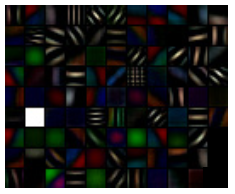
\includegraphics[width=0.4\linewidth]{images/4_max_norm}
\caption[]{Ein dominierender Filter ohne Max-Norm Regularisierung  \cite[siehe][]{Zeiler2014}}.
\label{fig:4_max_norm}
\end{figure}

 Abbildung \ref{fig:4_max_norm} zeigt einen weiteren Grund für die Notwendigkeit dieser Form der Regularisierung. Die Dominanz eines Filters über alle anderen kann effektiv verhindert werden \cite[vgl.][]{Zeiler2014}.




\subsection{Modellkapazität}
Beim Training großer Modelle mit hoher Kapazität ist \textit{Overfitting} von zentraler Bedeutung. \textit{Overfitting} beschreibt den Effekt eines kleiner werdender Fehlers auf den Trainingsdaten bei gleichzeitiger Verschlechterung der Performanz auf den Testdaten. Abbildung \ref{fig:4_overfitting} stellt diesen Effekt grafisch dar.

\begin{figure}[H]
\centering
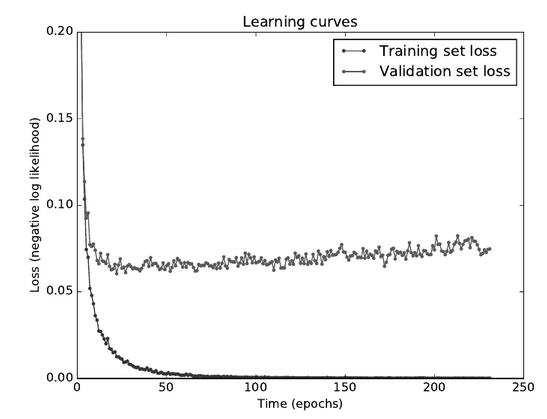
\includegraphics[width=0.4\linewidth]{images/4_overfitting}
\caption[]{\textit{Overfitting} am Beispiel des MNIST-Datensatzes \cite[siehe][Kap. 7.3, S. 216]{Bengio2015} }.
\label{fig:4_overfitting}
\end{figure}

Unter Model Restriktionen werden im Folgenden Methoden zusammengefasst, welche die Kapazität des Modells regulieren und damit aktiv versuchen \textit{Overfitting} zu verhindern.



\subsubsection{Early Stopping}
Die einfachste sehr häufig angewandte Methode aktiv \textit{Overfitting} zu verhindern, ist das sogenannte \textit{Early Stopping}. Diese Methode teilt die Trainingsmenge zuerst in zwei Teilmengen. Sie setzt somit einen Satz Validierungsdaten voraus \cite[vgl. im Folgenden][Kap. 7.3, S. 216 ff.]{Bengio2015}.

Beim \textit{Early Stopping} wird nun in regelmäßigen Abständen während des Trainings der Fehler auf den Validierungsdaten beobachtet. Verbessert sich dieser, werden die aktuellen Parameter des Modells gesondert gespeichert. Am Ende des Trainings werden nun nicht die aktuellsten Parameter zurück\-gegeben sondern diejenigen, welche den kleinsten Validierungsfehler erzeugten.
Anstelle eines lokalen Minimums über den Trainingsdaten wird so ein lokales Minimum des Validierungsfehlers gesucht. Das Training stoppt, sobald sich der Validierungsfehler über mehrere Epochen nicht verbessert hat. Die Kapazität des Modells wird dahingehend beschränkt, dass die Trainingszeit limitiert ist.

Bei der $L^2$-Regularisierung wurde beobachtet, dass Parameter in Richtungen hoher Krümmung hinsichtlich der Zielfunktion weniger stark reguliert werden als andere. Diese Beobachtung lässt eine Ähnlichkeit zum \textit{Early Stopping} erkennen, da die Parameter in Verbindung mit hoher Krümmung relativ zu den anderen Parametern früher im Trainingsprozess gelernt werden.

\subsubsection{Parameteranzahl limitieren}
Ganz Intuitiv lässt sich die Kapazität des Modells durch Vereinfachung bzw. Verkleinerung und somit einer Verringerung der Parameter regulieren. Im Umfeld des Deep Learning werden grundsätzlich zwei verschiedene Methoden beschrieben: Teilen der Parameter (\textit{Parameter Sharing}) und Verbindungen zwischen Merkmalen. \\

\textit{Parameter Sharing} \\
Diese Methode ist am meisten verbreitet in CNNs und Grundlage für die großen Erfolge im maschinellen Lernen und Deep Learning. CNNs berechnen an verschiedenen Stellen des Eingabebeispiels mit den selben Parametern eine gewichtete Summe, was der algebraischen Faltung entspricht \cite[vgl.][]{LeCun1998}. 
Durch Parameter Sharing ist es möglich große neuronale Netze zu trainieren ohne die Trainingsmenge entsprechend zu vergrößern. Damit sind CNNs ein Paradebeispiel für die Integration von Expertenwissen in einem neuronalen Netz \cite[vgl.][Kap 7.8, S. 224]{Bengio2015}. \\

\textit{Verbindungen zwischen Merkmalen limitieren} \\
Diese Methode verfolgt ebenso das Ziel Parameter zu reduzieren, wählt allerdings einen anderen Ansatz. Anstatt die Eingabe nur in über\-lapp\-ende rezeptive Felder zu unterteilen und mit den selben Parametern zu gewichten, werden zusätzlich die unterschiedlichen Dimensionen der Eingabe (z. B. RGB-Kanäle) überlappend aufgeteilt. Die bekannte Verbindungsmatrix von \textit{LeNet 5} ist zur Veranschaulichung in Abbildung \ref{fig:4_connections} dargestellt. 

\begin{figure}{H}
\centering
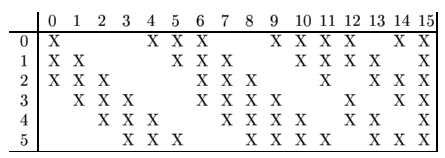
\includegraphics[width=0.4\linewidth]{images/4_connections}
\caption[]{Verbindungsmatrix der Merkmale bzw. \textit{Feature-Maps} (Zeilen) mit den dazugehörigen Gewichten bzw. Faltungsmasken (Spalten) zweier aufeinanderfolgenden Schichten \cite[siehe][]{LeCun1998}}.
\label{fig:4_connections}
\end{figure}

Neben der Reduktion von Parametern erlaubt dies auch eine bessere Extraktion unabhängiger Merkmale \cite{LeCun1998}. Darüber hinaus bedient sich die Architektur von \cite{Krizhevsky2012} derselben Methode zwecks Parallelisierung des Netzes auf mehrere Rechenkerne (GPUs), wie Abbildung \ref{fig:4_Kriz} zeigt.

\begin{figure}[H]
\centering
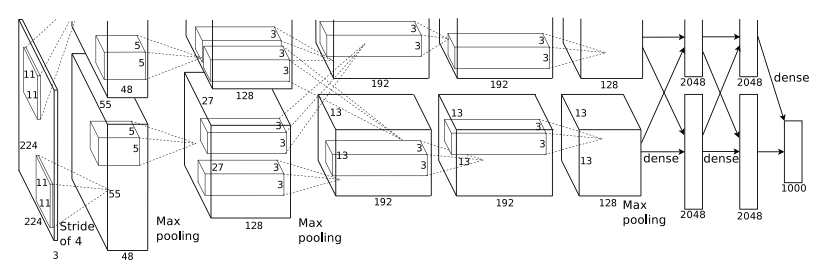
\includegraphics[width=0.9\linewidth]{images/4_Kriz}
\caption[]{Architektur für \textit{ImageNet 2012} mit limitierten Verbindungen zwischen \textit{Feature-Maps}zwecks Parallelisierung  \cite[siehe][]{Krizhevsky2012}}.
\label{fig:4_Kriz}
\end{figure}


\subsubsection{Dropout}
\label{ch:dropout}
Dropout von \cite{Hinton2012} bezeichnet im eigentlichen Sinn eine Methode mehrere kleinere Modelle zu lernen und die verschiedenen Ausgaben zu kombinieren (\textit{Model Averaging}). Das interessante an der Dropout Methode ist, dass dies in einem neuronalen Netz und gleichzeitig geschieht \cite[vgl.][]{Srivastava2014}.

Den Ursprung von Dropout liegt darin, MLPs mit wenigen Trainingsdaten zu trainieren, was typischerweise in \textit{Overfitting} resultiert. Die Idee ist es die Architektur des Netzes im Training zufällig für jedes Trainingsbeispiel zu verändern um Abhängigkeiten (\textit{co-adaptions}) extrahierter Merkmale zu vermeiden \cite[vgl.][]{Hinton2012}. Dazu werden zufällig einzelne Neuronen deaktiviert. Dieses Grundprinzip ist in Abbildung \ref{fig:4_dropout} dargestellt. Um den Gradienten richtig zu berechnen ist es wichtig, dass im Backpropagation beim \textit{Backward Pass} die deaktivierten Neuronen ebenso deaktiviert bleiben.

Wird die zufällige Deaktivierung weggelassen, existiert ein trainiertes Netz, welches implizit mehrere Modelle kombiniert und so eine deutliche Verbesserung gegenüber bestehenden Regularisierungs-Methoden hinsichtlich \textit{Overfitting} darstellt \cite[vgl.][]{Srivastava2014}. Damit durch die Kombination der Modelle die Parameter im Betrieb nicht zu groß sind, müssen diese mit ${1-p}$ skaliert werden. 

Als Hyperparameter muss für Dropout lediglich die Wahrscheinlichkeit $p$ ein Neuron zu deaktivieren angegeben werden. Typische Werte reichen von $0.1$ bis $0.5$ (vgl. \cite{Krizhevsky2012}, \cite{Srivastava2014} oder \cite{Simonyan2014}).

Bei Verwendung von Standardinitialisierung in Verbindung mit ReLu-Funk\-tionen muss darauf geachtet werden, dass die Neuronen positive Ausgaben erzeugen um ebenso positive Gradienten für das Lernen zu bekommen. Dies kann mittels Schwellwert $b=1$ oder einer hinreichend große Varianz erreicht werden \cite[vgl.][]{Hinton2012}.

Dropout kann auch bestehende gut funktionierende Netze verbessern. Da die effektive Kapazität durch Dropout verringert wird, ist es sinnvoll die Anzahl existierender Neuronen $n$ auf $\frac{n}{1-p}$ zu erhöhen \cite[vgl.][]{Srivastava2014}.\\ 

\begin{figure}
\centering
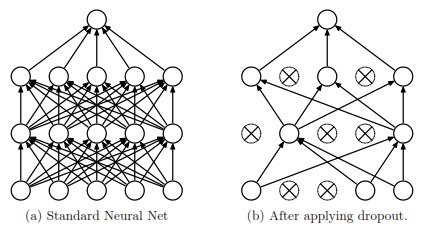
\includegraphics[width=0.6\linewidth]{images/4_dropout}
\caption[]{Schematische Darstellung eines gewöhnlichen MLP (links) und eines Dropout-MLP (rechts) \cite[siehe][]{Srivastava2014}}.
\label{fig:4_dropout}
\end{figure}			
	
Aufgrund der Tatsache, dass CNNs die Modellkapazität durch \textit{Parameter Sharing} bereits stark regulieren, ist Dropout in Convolution-Layer nicht so effektiv als in Hidden-Layer \cite[vgl.][]{Hinton2012}.	
			
\subsection{Erweitern der Trainingsdaten}
Die Kapazität eines Modells ist im Allgemeinen eine relative Größe hinsichtlich der zur Verfügung stehenden Trainingsmenge. Damit lässt sich das Problem des \textit{Overfittings} auch umgekehrt formulieren und anstatt die Kapazität zu regulieren, die Menge an Trainingsdaten erhöhen. Diese Methode wird häufig als \textit{Data Augmentation} bezeichnet und umfasst drei Bereiche: Affine Transformationen, Elastische Transformationen und Additives Rauschen.

Diese Formen der Regularisierung haben oftmals großen Einfluss auf die Performanz des Systems hinsichtlich Invarianzen und müssen deshalb beim Vergleich unterschiedlicher Algorithmen und Lernmaschinen berücksichtigt werden.
\cite[vgl.][Kap. 7.5, S. 210 f.]{Bengio2015}



\subsubsection{Affine Transformationen}
Affine Transformationen können die Generalisierung des Netzes immense verbessern. Die Idee ist es Eingaben so zu verändern, dass gewünschte Invarianzen besser trainiert werden. Dies ist auch dann von Vorteil, wenn das Modell selbst bereits gewisse Invarianzen beherbergt, wie beispielsweise die Translationsinvarianz von CNNs. So finden affine Transformationen beispielsweise Anwendung im Training von \textit{LeNet 5} von \cite{LeCun1998} und im \textit{AlexNet} von \cite{Krizhevsky2012}.
Eine analytische Methode \textit{Data Augmentation} in den Trainingsprozess einzubauen beschreibt \cite{Simard92} im Tangent-Prop Algorithmus.


\subsubsection{Elastische Transformationen}
Elastische Transformationen erweitern das Set an verfügbaren affinen Operationen und verbessert die Generalisierung dadurch weiter. 
Die Vorgehensweise beschreibt zuerst die Generierung eines Vektorfelds pro Dimension, welches zufällige Verschiebungen der einzelnen Eingabemerkmale (Pixel) beschreibt. Die generierten Felder werden anschließend mit einem Gauss-Kern gefaltet bzw. weichgezeichnet und auf die originale Eingabe angewandt \cite[vgl.][]{Simard2003}.
Das Ergebnis elastischer Transformationen ist in Abbildung \ref{fig:4_elastic} dargestellt.

\begin{figure}
\centering
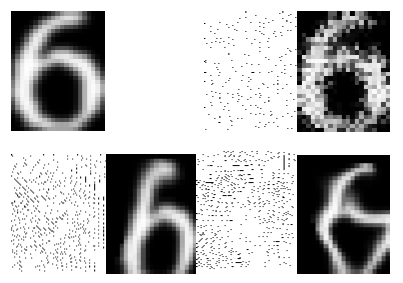
\includegraphics[width=0.5\linewidth]{images/4_elastic}
\caption[]{Originale Eingabe (oben links) und drei Beispiele elastisch veränderter Eingaben mit zugehörigem Vektorfeld \cite[siehe][]{Simard2003}}.
\label{fig:4_elastic}
\end{figure}


\subsubsection{Additives Rauschen}
Eine weitere Möglichkeit das System robuster zu machen, ist das Training mit additivem Rauschen. So korrumpiert beispielsweise \cite{Vincent2008} die Eingabe zu einem gewissen Grad mit additiven Rauschen, Maskierung oder \textit{Salt-and-pepper} und konstruiert damit einen \textit{Denoising Autoencoder} (DAE). Mehrere DAEs bilden sogenannte \textit{Stacked Denoising Autoencoder} und schließen damit die Lücke zu den beschränkten Boltzmann-Maschinen und (DBNs) im Bereich des unüberwachten Vortrainings tiefer Netze \cite[vgl.][]{Vincent2010}.

Gerade die Maskierung einzelner Merkmale im Eingaberaum liefert die Grundlage für das spätere Dropout, welches sowohl für die Hidden-Layer als auch im Input-Layer geeignet ist und die Generalisierung deutlich verbessern kann \cite[vgl.][]{Srivastava2014}.


\section{Visualisierungsmethoden}
Gerade die Verbindung von Bilderkennung mit CNNs macht Visualisierungsmethoden besonders attraktiv, da sich gewisse Verhaltensweisen des neuronalen Netzes so besser verstehen lassen.
Die meisten der vorgestellten Methoden haben das Ziel der Kritik, \textit{Features} aus neuronalen Netzen lassen sich nicht interpretieren, entgegenzuwirken \cite[vgl.][]{Zeiler2014}.

\subsection{Primitiv}

Die einfachste Möglichkeit ist die Visualisierung der Ausgabe bzw. der Parameter und wird deshalb als primitiv bezeichnet. Dennoch können diese Techniken wichtige Einblicke gewähren.

\subsubsection{Neuronen-Aktivierung}

Die Visualisierung der Ausgabe eines \textit{AlexNet} von \cite{Krizhevsky2012} ist in Abbildung \ref{fig:4_output} (links) dargestellt. Die Eingabe ist ein Bild einer Katze. Es fällt sofort auf, dass die Aktivierungen sehr dünnbesetzt (\textit{sparse}) sind, was letztendlich auf die ReLu-Funktionen zurückzuführen ist \cite[vgl.][]{Glorot2011}.

\begin{figure}
\centering
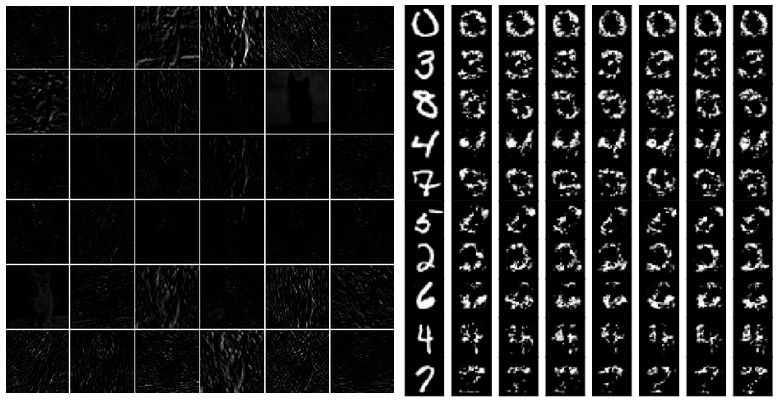
\includegraphics[width=0.6\linewidth]{images/4_output}
\caption[]{Aktivierungen des \textit{AlexNet} nach erstem Layer (links)  \cite[siehe][]{Kaparthy2014} und Rekonstruktionen eines Autoencoders (rechts) \cite[siehe][]{Vincent2010}}.
\label{fig:4_output}
\end{figure}

Diese Visualisierungstechnik kann in mehrerer Hinsicht unterstützen. Einerseits können so tote Neuronen identifiziert werden (vgl. \textit{Dying ReLu}-Effekt in \cite{Maas2013}). Andererseits kann überprüft werden, ob die Aktivierungen die gewünschte \textit{Sparsity} und Lokalität aufweisen.
Hinsichtlich Autoencoder und unüberwachtem Vortraining kann darüber hinaus interessant sein, die Aktivierung bzw. Ausgabe des Netzes zu visualisieren, da diese der Rekonstruktion der Eingabe entsprechen. Abbildung \ref{fig:4_output} (rechts) zeigt derartige Rekonstruktionen auf dem MNIST-Datensatz.

\subsubsection{Faltungskerne}
%http://eric-yuan.me/cnn/

Eine weitere einfache Möglichkeit Informationen über das CNN zu erhalten ist die Visualisierungen der gelernten Filtermasken. Abbildung \ref{fig:4_kernel} zeigt die Faltungskerne des ersten Layers eines trainierten \textit{AlexNet}. 

\begin{figure}[H]
\centering
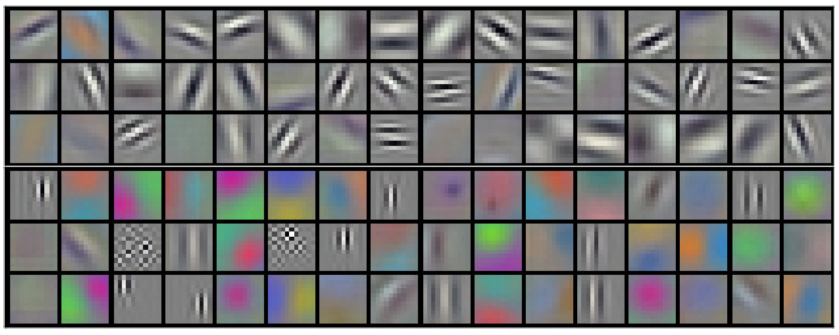
\includegraphics[width=0.5\linewidth]{images/4_kernel}
\caption[]{Die Faltungskerne des ersten Layers eines trainierten \textit{AlexNet}  \cite[siehe][]{Krizhevsky2012}}.
\label{fig:4_kernel}
\end{figure}

Trainierte Netze haben typischerweise glatte, Gabor-Filter ähnliche Filtermasken. Verrauschte Filtermasken können hingegen ein Indikator dafür sein, dass das Netz nicht ausreichend konvergiert ist oder auf fehlende Regularisierung und damit verbundenem \textit{Overfitting} \cite[vgl.][]{Kaparthy2014}.     


\subsection{Gradientenbasiert}

Eine weitere Klasse prominenter Visualisierungsmethoden arbeiten auf Basis des Backpropagation-Algorithmus. Dies bedeutet, dass sie sich der Fehlerrückführung (\textit{Backward Pass}) bedienen und diese zur Visualisierung verwenden.

\subsubsection{Neuronen-Visualisierung}
Die erste Methode ist die sogenannte Deconvnet-Visualisierung von \cite{Zeiler2014}. Diese Form der Visualisierung kann als Neuronen-Visualisierung bezeichnet werden, da letztlich Aktivierungen einzelner Neuronen visualisiert werden. Grundidee des Verfahrens ist es, einzelne Aktivierungen im Netz im Eingaberaum sichtbar zu machen. Dazu wird ein bestimmtes Neuron, eine bestimmte \textit{Feature-Map} ausgewählt und die Aktivierungen über die gesamte Testmenge gemessen. Die Beispiele, mit den höchsten Aktivierungen werden gespeichert. Die Visualisierung nimmt diese Beispiele im Anschluss und rekonstruiert die erzeugten Aktivierungen, indem alle anderen \textit{Feature-Maps} dieses Layers auf Null gesetzt werden. Für die Rekonstruktion $R$ der Aktivierung selbst wird im Grunde die Fehlerrückführung des Backpropagation-Algoritmus verwendet. Damit gilt in einem Convolution-Layer die Gleichung \ref{eq:zeiler1} zur Rekonstruktion einer Feature-Map.

\begin{equation}
\label{eq:zeiler1}
R^l_j = \sum_{i = 0}^{n} \hat{R}^{l+1}_{i} \ast rot180(W_{ij})
\end{equation}

Im Unterschied zur Berechnung des Gradienten im Backpropagation, wird bei diesem Verfahren die Aktivierungsfunktionen nicht abgeleitet und stattdessen die Aktivierungsfunktion $\phi$ selbst mit der Rekonstruktion $R^{l+1}$ im Sinne des \textit{Forward Pass} berechnet. Formel \ref{eq:zeiler2} verdeutlicht diesen Zusammenhang für den Layer $l$.

\begin{equation}
\label{eq:zeiler2}
\hat{R}^{l+1}_i = \phi_l(R^{l+1}_i)
\end{equation}

Eine weitere Besonderheit stellen die Pooling-Layer dar, da diese im Prinzip nicht umkehrbar sind. Die von \cite{Zeiler2014} vorgeschlagene Methode sieht deshalb lediglich die Variante Max-Pooling vor und verbietet alle anderen Pooling-Verfahren. Max-Pooling bietet den Vorteil, dass im \textit{Forward Pass} die Stellen der Maxima vermerkt werden.

\begin{figure}
\centering
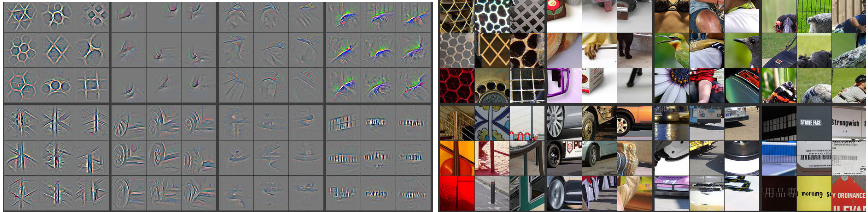
\includegraphics[width=0.9\linewidth]{images/4_zeiler}
\caption[]{Mit Deconvnet rekonstruierte Aktivierungen im dritten Layer (links) und dazugehörige Originale Eingabebilder (rechts) \cite[siehe][]{Zeiler2014}}.
\label{fig:4_zeiler}
\end{figure}

Acht ausgewählte Neuronen im dritten Layer mit den jeweiligen zur höchsten Aktivierung korrespondierenden Eingabebildern sind in Abbildung \ref{fig:4_zeiler} dargestellt.

\subsubsection{Saliency-Visualisierung}
%Gerneralized
Die sogenannte Saliency-Visualisierung von \cite{Simonyan2013} ist im Grunde dem Deconvnet-Verfahren sehr ähnlich. Es unterscheidet sich allerdings in einem zentralen Punkt. 
Während das Verfahren von \cite{Zeiler2014} Veränderungen im Vergleich zum Backpropagation vornimmt, hält sich dieses Verfahren strikt an die Fehlerrückführung und berechnet damit die Ableitungen der Aktivierungsfunktionen wie Formel \ref{eq:simonyian} zeigt. 

\begin{equation}
\label{eq:simonyian}
\hat{R}^{l+1}_i = R^{l+1}_i \circ \phi^{'}(z_i)
\end{equation}

Dies bietet den Vorteil, dass sich das Verfahren so sowohl auf die Convolution-Layer als auch die Hidden-Layer anwenden lässt. Dies lässt sich damit begründen, dass das Verfahren im ursprünglichen Sinn einzelne Klassen im Eingaberaum visualisiert \cite[vgl.][]{Simonyan2013}.


\begin{figure}
\centering
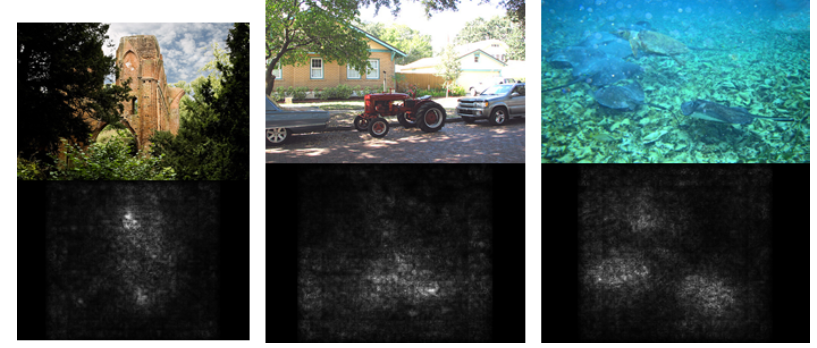
\includegraphics[width=0.6\linewidth]{images/4_simonyan}
\caption[]{Originale Eingabebilder (oben) und dazu gehörige \textit{Siliency-Maps} (unten) \cite[siehe][]{Simonyan2013}}.
\label{fig:4_simonyan}
\end{figure}

Abbildung \ref{fig:4_simonyan} zeigt die Technik angewandt auf Beispiele aus dem \textit{ImageNet}-Datensatz. Die \textit{Saliency-Map} zeigt die Rekonstruktion der entsprechenden Aktivierung im Output-Layer. 

\subsection{Nachverarbeitung}
%CS Workshop
%t-SNE before and after training
%Feature Extraction
Methoden im Bereich Nachverarbeitung sind dadurch charakterisiert, dass ein trainiertes MLP bzw. CNN lediglich zur Erzeugung von Merkmalsvektoren bzw. zur Berechnung von Ausgaben herangezogen wird. Diese Art der Visualisierung beschränkt sich demnach auf den Kontext und betrachtet das Netz als \textit{Blackbox} bzw. als Funktion $h(x)$.


\subsubsection{t-SNE}

t-Distributed Neigbor Embedding (t-SNE) beschreibt ein von \cite{Laurens2008} entwickeltes Optimierungsverfahren zur Dimensionsreduktion. Es verbessert das klassische SNE-Verfahren insofern, dass die Gradienten für die Optimierung einfacher zu berechnen sind und anstelle einer Gauß- eine Student-t-Verteilung als Ähnlichkeitsmaß im niedrigdimensionalen 2D bzw. 3D Zielraum verwendet wird \cite[vgl.][]{Laurens2008}. Grundmechanismus von t-SNE ist die Minimierung des Unterschieds zweier Wahrscheinlichkeitsverteilungen (Kullback-Leibler-Divergenz) \textemdash \space Der Wahrscheinlichkeitsverteilung von Paaren im hochdimensionalen $P$ Raum sowie der im niedrigdimensionalen Raum $Q$. Damit ergibt sich die zu minimierende Zielfunktion $C$ in Formel \ref{eq:tsne}.


\begin{equation}
\label{eq:tsne}
C = KL(P||Q) ) = \sum_{i}^{} \sum_{j}^{} p_{ij} log(\frac{p_{ij}}{q_{ij}})
\end{equation}


\begin{figure}
\centering
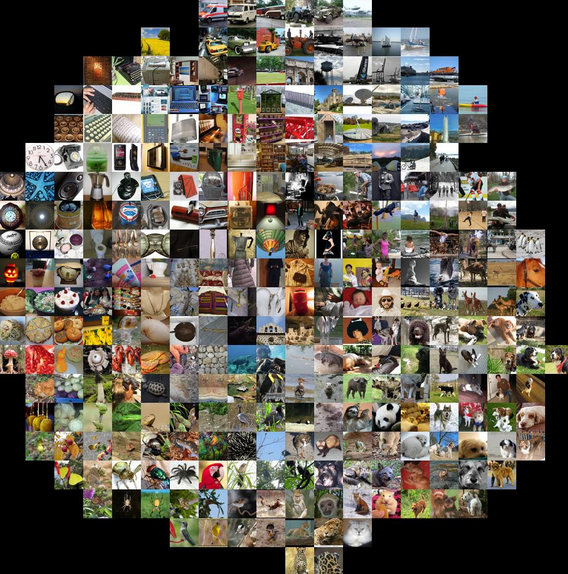
\includegraphics[width=0.5\linewidth]{images/4_t_sne}
\caption[]{t-SNE Einbettung einer Auswahl an \textit{ImageNet}-Bildern auf Basis der Aktivierung des letzten Layers im \textit{AlexNet} (Bild: Laurens van der Maaten, Facebook AI Research)}.
\label{fig:4_t_sne}
\end{figure}


Grundsätzlich können die von neuronalen Netzen erzeugten Merkmalsvektoren (\textit{Features}) auch mittels Hauptkomponentenanalyse (PCA) visualisiert werden. Die t-SNE unterscheidet sich von PCA allerdings in einigen zentralen Eigenschaften \cite[vgl. im Folgenden][]{Laurens2008}:

\begin{itemize}
\item Wenn ein Großteil der Varianz nicht in den ersten zwei bzw. drei Hauptkomponenten beschrieben ist, kann t-SNE bessere Ergebnisse liefern, da es versucht die gesamte Information abzubilden.
\item t-SNE ist im Vergleich zur PCA keine orthogonale lineare Transformation sondern eine nichtlineare Reduktion mit nicht zwingend orthogonalen Komponenten.
\item t-SNE findet aufgrund der nicht-konvexen Zielfunktion nicht immer zum globalen Minimum.
\item t-SNE ist optimiert hochdimensionale Daten auf maximal zwei bzw. drei Dimensionen zu reduzieren.
\end{itemize}



Abbildung \ref{fig:4_t_sne} zeigt die t-SNE 2D-Transformation des Merkmalsvektors vor dem Output-Layer eines \textit{AlexNet} auf Basis einer Teilmenge des \textit{ImageNet}-Datensatzes. Diese Art der Visualisierung zeigt, dass das CNN Merkmale extrahiert und darauf aufbauend relevante von irrelevanten Merkmalen trennen kann. Dies lässt sich sehr deutlich daran erkennen, dass inhaltlich ähnliche Bilder näher zusammen sind als andere und somit Kategorien oder Gruppen und nicht Hintergrund oder Färbung dominieren \cite[vgl.][]{Bell2015}.


\begin{figure}[t]
\centering
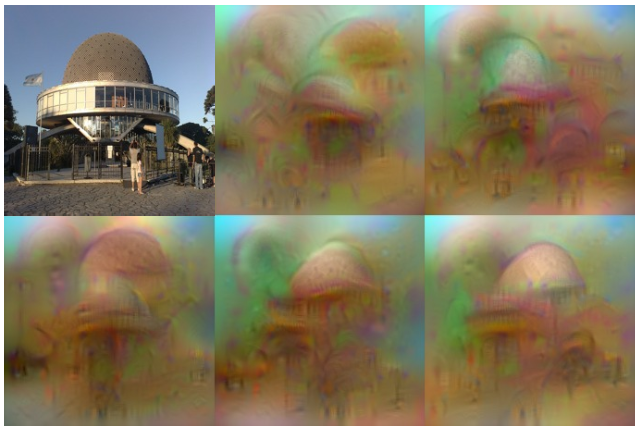
\includegraphics[width=0.6\linewidth]{images/4_inceptionism}
\caption[]{Mögliche Rekonstruktionen des originalen Eingabebilds (oben links) \cite[siehe][]{Simard2003}}.
\label{fig:4_inceptionism}
\end{figure}

\subsubsection{Inceptionism}
Ein weiteres Verfahren, welches als \textit{Inceptionism}\footnote{Das Kunswort \textit{Inceptionism} geht auf einen Blog-Eintrag von \textit{Research at Google} zurück (\url{http://googleresearch.blogspot.de/2015/06/inceptionism-going-deeper-into-neural.html} (26.08.2015)).} propagiert wird, wählt eine andere Herangehensweise. Dieses Verfahren versucht, ausgehende von einer Aktivierung bzw. eines Merkmalsvektors eines Layers, eine dazu passende Eingabe zu rekonstruieren. 
Das Grundverfahren um Merkmalsvektoren zu invertieren stammt von \cite{Mahendran2014}. Dieses Verfahren nimmt ein beliebiges Eingabebild $x_0$ und berechnet mittels eines trainierten CNN die Ausgabe $h_0 = h_l(x_0)$ in einem beliebigen Layer $l$. Ziel des Verfahrens ist es die Zielfunktion $C$ in Gleichung \ref{eq:incept} mit Regularisierer $R(x)$ zu minimieren und ausgehend von Rauschen ein optimales $x$ zu finden. 

\begin{equation}
\label{eq:incept}
C = ||h(x) - h_0||^2 + \lambda R(x)
\end{equation}

Der Regularisierer sorgt einerseits dafür, dass das optimale $x$ innerhalb eines für Bilder üblichen Intervalls $B = [-128,128]$ liegt (Formel \ref{eq:incept1}) und das resultierende Bild stückweise konstant ist (Formel \ref{eq:incept2}).

\begin{equation}
\label{eq:incept1}
R_1 = ||x||^6_6
\end{equation}

\begin{equation}
\label{eq:incept2}
R_2 = \sum_{i,j}^{} [(x_{i,j+1} - x_{ij})^2 + (x_{i+1,j} - x_{ij})^2)]^{\frac{1}{2}}
\end{equation}


Abbildung \ref{fig:4_inceptionism} zeigt fünf Optimierungen auf Basis des Eingabebilds oben links.


